\chapter{Projekt i implementacja aplikacji klienckiej oraz REST API}

\section{Funkcje aplikacji}

%TODO: krótki opis

\subsection{Diagram przypadków użycia}

\begin{figure} [H]
	\centering
	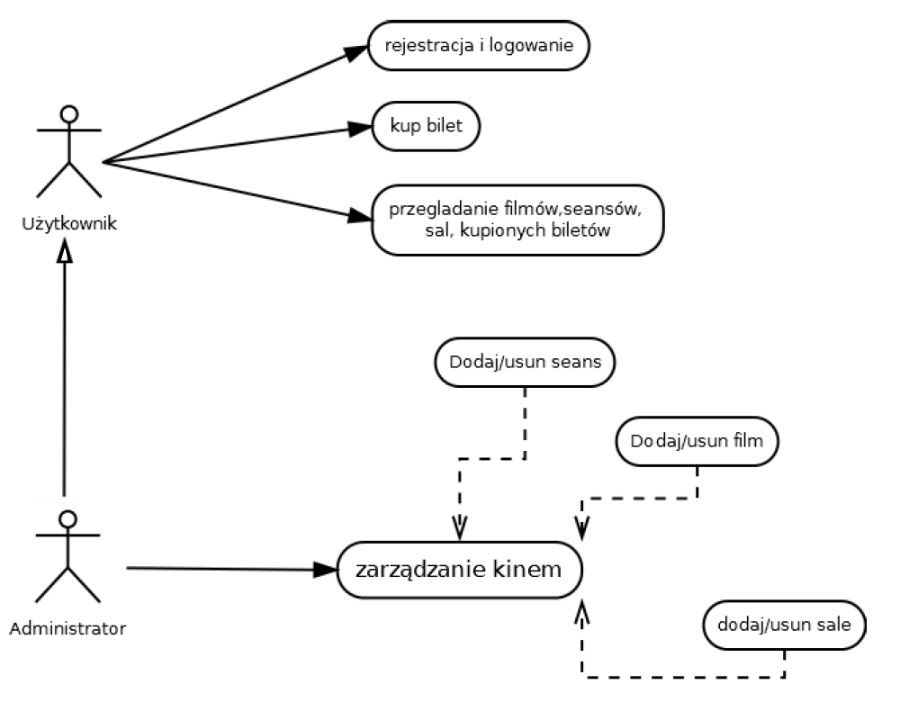
\includegraphics[width=0.6\linewidth]{rozdzial05/diagram.png}
	\caption{Diagram przypadków użycia}
	\label{fig:schem}
\end{figure}

Użytkownik:
\begin{itemize}
	\item tworzenie nowego konta (podanie loginu, hasła itp.);
	\item logowanie;
	\item przeglądanie filmów, seansów, kupionych biletów;
	\item kupowanie biletów.
\end{itemize}

Administrator:
\begin{itemize}
	\item te same funkcjonalności co użytkownik;
	\item dodawanie/usuwanie/edytowanie seansów;
	\item dodawanie/usuwanie/edytowanie filmów;
	\item dodawanie/usuwanie/edytowanie dostępnych sal.
\end{itemize}

\subsection{Scenariusz wybranych przypadków użycia}

W poniższych tabelach umieszczone zostały scenariusze wybranych przypadków użycia.

\begin{table}[H]
	\begin{tabularx}{\textwidth}{ |l|X| }
		\hline 
		Przypadek użycia & Rejestracja  \\ 
		\hline 
		Opis & Funkcja umożliwiająca założenie konta w systemie \\ 
		\hline 
		Warunki początkowe & Brak konta \\ 
		\hline 
		Warunki końcowe & System utworzył konto lub odrzucił żądanie  \\ 
		\hline 
		Przebieg podstawowy & 1. Użytkownik podaje swoje dane (login, hasło itp.) \\ 
		& 2. System sprawdza czy login nie jest zajęty \\
		& 3. Jeśli login jest wolny, skok do pkt 6. \\
		& 4. Wyświetlenie komunikatu o błędach \\
		& 5. Skok do pkt 1. \\
		& 6. Zakończenie rejestracji \\
		\hline 
	\end{tabularx} 
    \caption{Scenariusz rejestracji}
\label{tab:scen1}   
\end{table}

\begin{table}[H]
	\begin{tabularx}{\textwidth}{ |l|X| }
		\hline 
		Przypadek użycia & Logowanie  \\ 
		\hline 
		Opis & Funkcja umożliwiająca użytkownikom uzyskanie dostępu do systemu \\ 
		\hline 
		Warunki początkowe & Posiadanie własnego konta \\ 
		\hline 
		Warunki końcowe & System autoryzował, bądź odrzucił użytkownika  \\ 
		\hline 
		Przebieg podstawowy & 1. Użytkownik podaje swój login i hasło \\ 
		& 2. System wyszukuje użytkownika \\
		& 3. Jeśli użytkownik zostanie zweryfikowany, skok do pkt 6. \\
		& 4. Wyświetlenie komunikatu o błędach \\
		& 5. Skok do pkt 1. \\
		& 6. Zakończenie logowania \\
		\hline 
	\end{tabularx} 
	\caption{Scenariusz logowania}
	\label{tab:scen2}   
\end{table}

\begin{table}[H]
	\begin{tabularx}{\textwidth}{ |l|X| }
		\hline 
		Przypadek użycia & zarządzanie kinem  \\ 
		\hline 
		Opis & Funkcja umożliwiająca pracownikom zarządzanie kinem \\ 
		\hline 
		Warunki początkowe & Funkcja dostępna tylko dla zalogowanych pracowników \\ 
		\hline 
		Warunki końcowe & Dokonanie zmiany w systemie  \\ 
		\hline 
		Przebieg podstawowy & 1. Pracownik uruchamia aplikację zarządzania kinem \\ 
		& 2. Wywołanie odpowiedniego przypadku w zależności od wybranej akcji do wykonania \\
		& 3. Jeżeli wybrano "Dodanie filmu", wywołanie przypadku "Dodanie filmu". Skok do pkt 8. \\
		& 4. Jeżeli wybrano "Dodanie seansu", wywołanie przypadku "Dodanie seansu". Skok do pkt 8. \\
		& 5. Jeżeli wybrano "Usuwanie filmu", wywołanie przypadku "Usuwanie filmu". Skok do pkt 8. \\
		& 6. Jeżeli wybrano "Usuwanie seansu", wywołanie przypadku "Usuwanie seansu". Skok do pkt 8. \\
		& 7. Jeżeli wybrano "Dodawanie sali", wywołanie przypadku "Dodanie sali". Skok do pkt 8. \\
		& 8. Zakończenie procesu \\
		\hline
		Przebieg alternatywny & 1. Pracownik wchodzi na stronę zarządzania kinem. \\
		& 2. Wywołanie odpowiedniego przypadku w zależności od wybranej akcji do wykonania \\
		& 3. Pracownik wylogował się z systemu \\
		& 4. zakończenie procesu. \\
		\hline 
	\end{tabularx} 
	\caption{Scenariusz zarządzania kinem}
	\label{tab:scen3}   
\end{table}

\section{Realizacja wybranych funkcjonalności aplikacji}

Aplikacja internetowa powstała z wykorzystaniem platformy programistycznej Angular 2. Jest to framework odpowiedzialny za tworzenia aplikacji po stronie klienta. Do zaprogramowania części funkcjonalnej aplikacji wykorzystuje on TypeScript czyli wolny i otwartoźródłowy język programowania stworzony przez firmę Microsoft jako nadzbiór języka JavaScript. Umożliwia on opcjonalne statyczne typowanie oraz programowanie zorientowane obiektowo oparte na klasach. TypeScript jest nadzbiorem JavaScript, a więc potencjalnie każdy program napisany w języku JavaScript jest poprawnym programem TypeScript. Aplikacje napisane w TypeScript kompilują się bezpośrednio do języka JavaScript. Poniżej znajdują się przykładowe fragmenty kodu napisane w tym języku odpowiedzialne za komunikację z API bazy danych.  

\lssetdef
\lstinputlisting[captionpos=b,caption={Implementacja funkcji GET po stronie aplikacji},label={lst:Get},basicstyle={\footnotesize\ttfamily}]{rozdzial05/GET.txt}

\lstinputlisting[captionpos=b,caption={Implementacja funkcji POST po stronie aplikacji},label={lst:Post},basicstyle={\footnotesize\ttfamily}]{rozdzial05/POST.txt}

\subsection{Interfejs aplikacji}

Aplikacja została napisana tak aby blokować widok niedozwolonych operacji jeśli użytkownik nie ma odpowiednich uprawnień. Poniżej znajdują się zrzuty ekranu widoku interfejsu z konta administracyjnego. 

\begin{figure} [H]
	\centering
	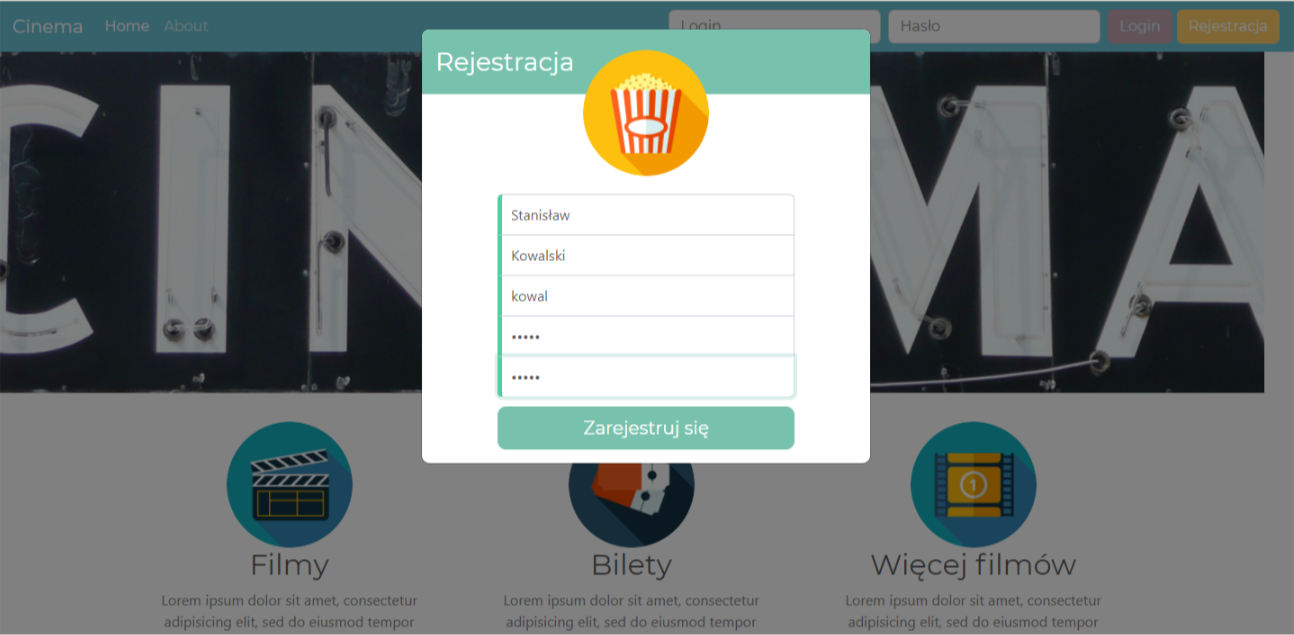
\includegraphics[width=1\linewidth]{rozdzial05/interfejs/rejestracja.png}
	\caption{Rejestracja użytkownika}
	\label{fig:screen1}
\end{figure}


\begin{figure} [H]
	\centering
	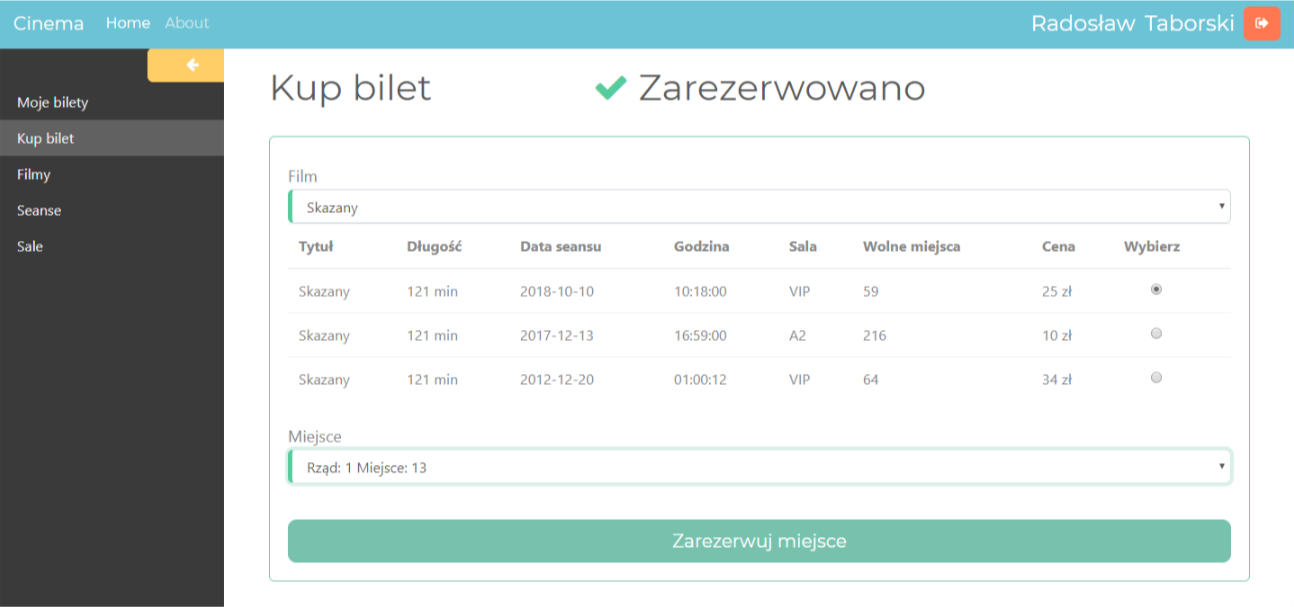
\includegraphics[width=1\linewidth]{rozdzial05/interfejs/kupBilet.png}
	\caption{Rezerwacja biletów}
	\label{fig:screen2}
\end{figure}

\begin{figure} [H]
	\centering
	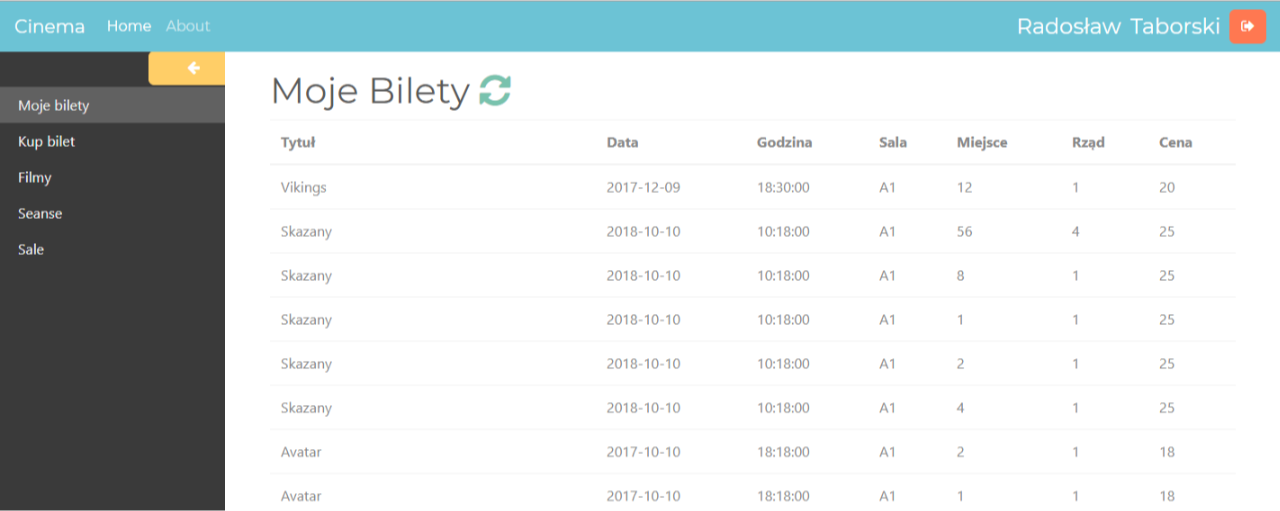
\includegraphics[width=1\linewidth]{rozdzial05/interfejs/mojeBilety.png}
	\caption{Widok biletów zarezerwowanych przez użytkownika}
	\label{fig:screen3}
\end{figure}

\begin{figure} [H]
	\centering
	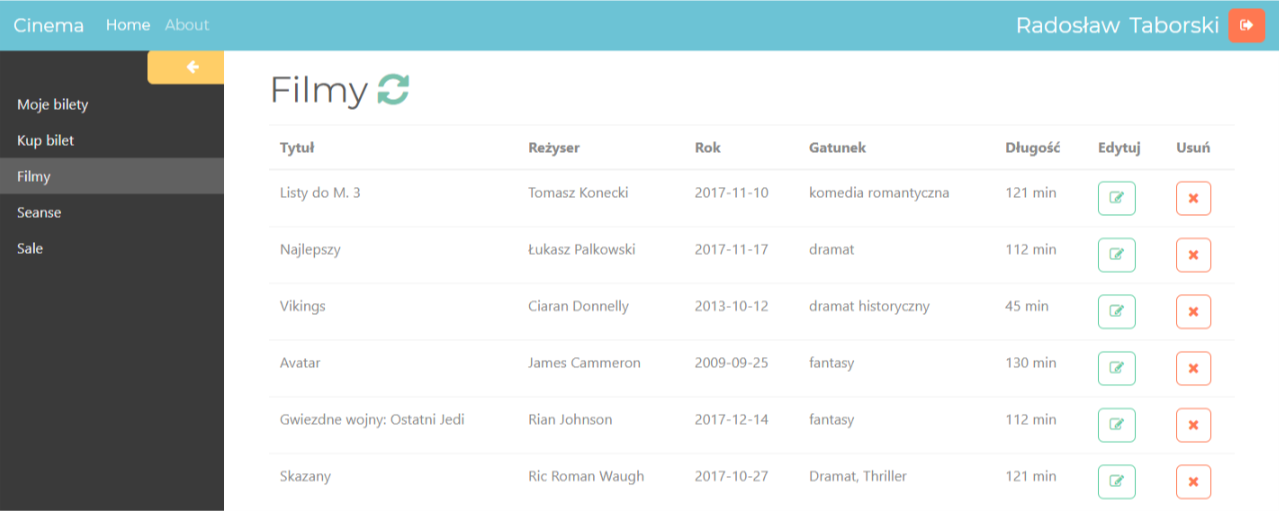
\includegraphics[width=1\linewidth]{rozdzial05/interfejs/filmy.png}
	\caption{Widok filmów dostępnych w kinie}
	\label{fig:screen4}
\end{figure}

\begin{figure} [H]
	\centering
	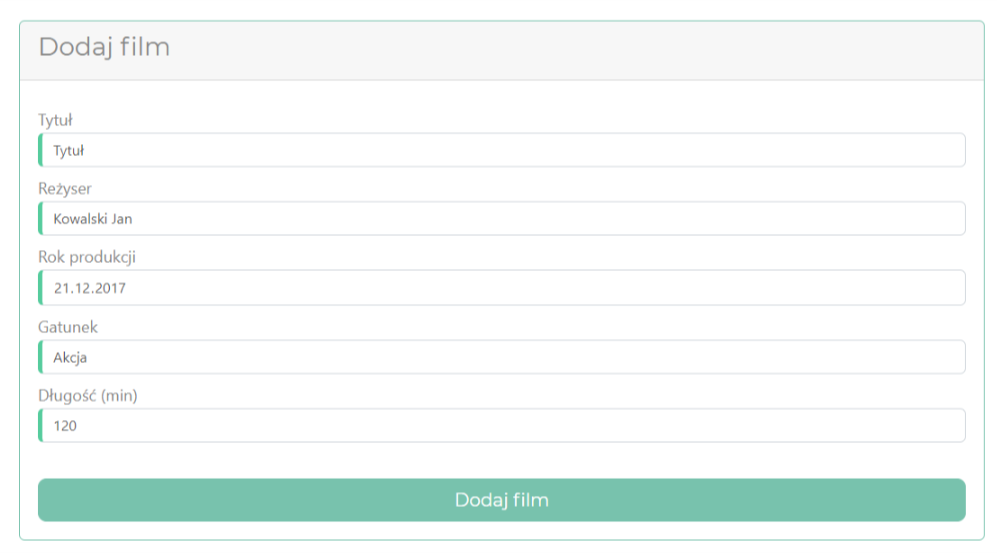
\includegraphics[width=1\linewidth]{rozdzial05/interfejs/dadajFilm.png}
	\caption{Dodawanie nowego filmu}
	\label{fig:screen5}
\end{figure}

\begin{figure} [H]
	\centering
	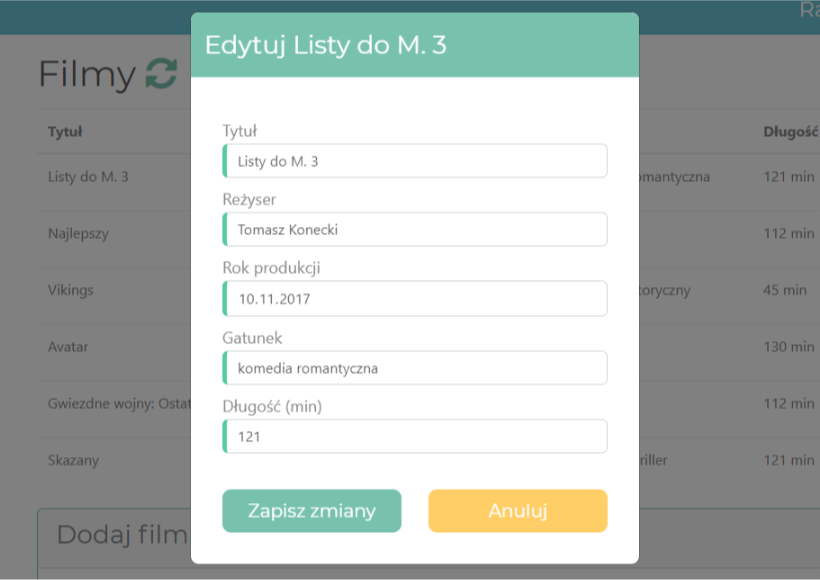
\includegraphics[width=1\linewidth]{rozdzial05/interfejs/edytujFilm.png}
	\caption{Edycja filmu}
	\label{fig:screen6}
\end{figure}

\begin{figure} [H]
	\centering
	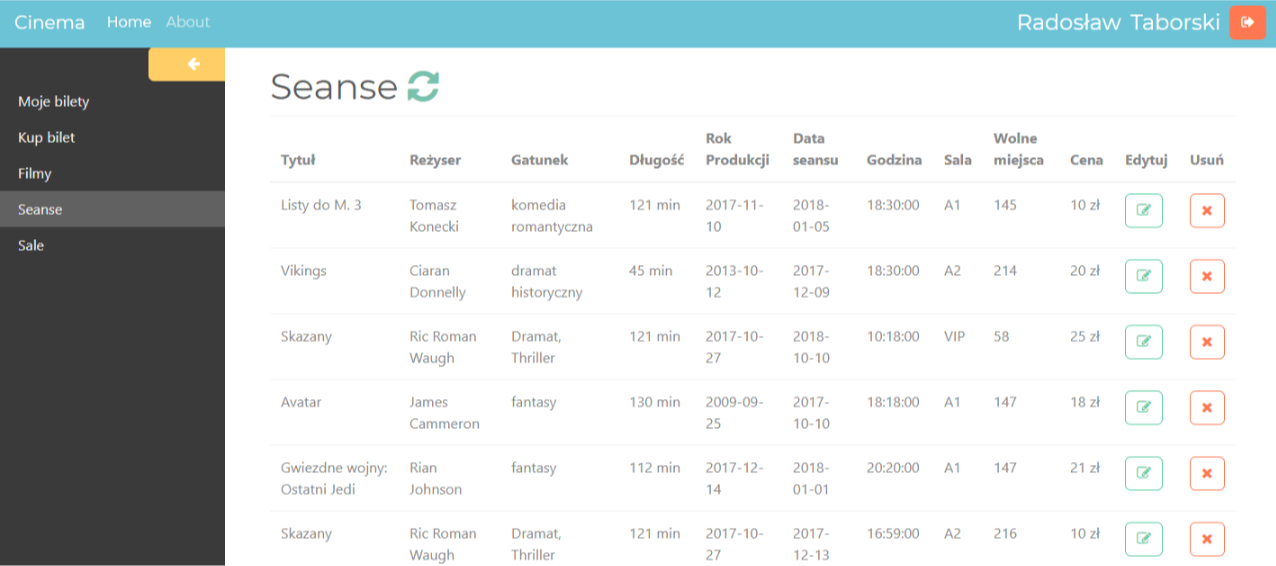
\includegraphics[width=1\linewidth]{rozdzial05/interfejs/seanse.png}
	\caption{Widok seansów dostępnych w kinie}
	\label{fig:screen7}
\end{figure}

\begin{figure} [H]
	\centering
	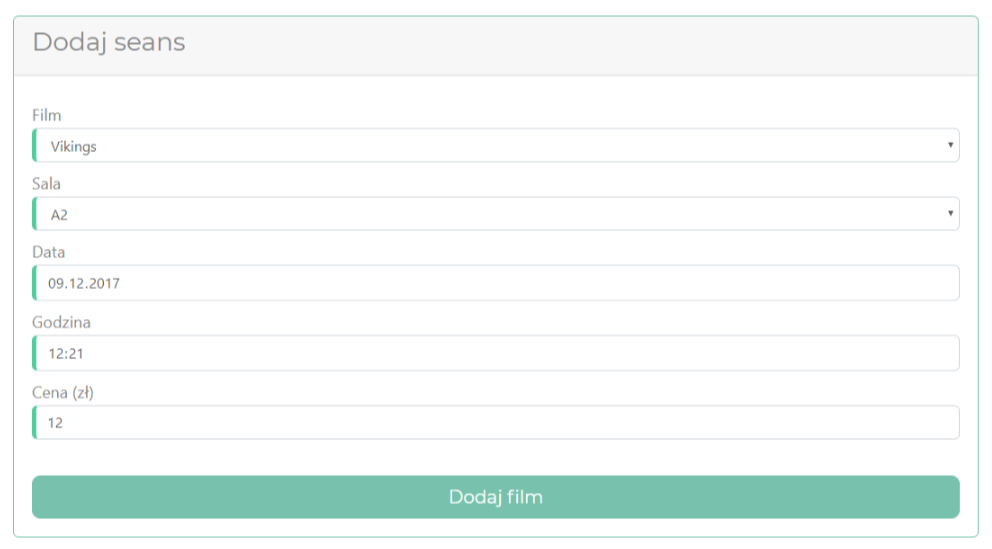
\includegraphics[width=1\linewidth]{rozdzial05/interfejs/dodajSeans.png}
	\caption{Dodawanie seansu}
	\label{fig:screen8}
\end{figure}

\begin{figure} [H]
	\centering
	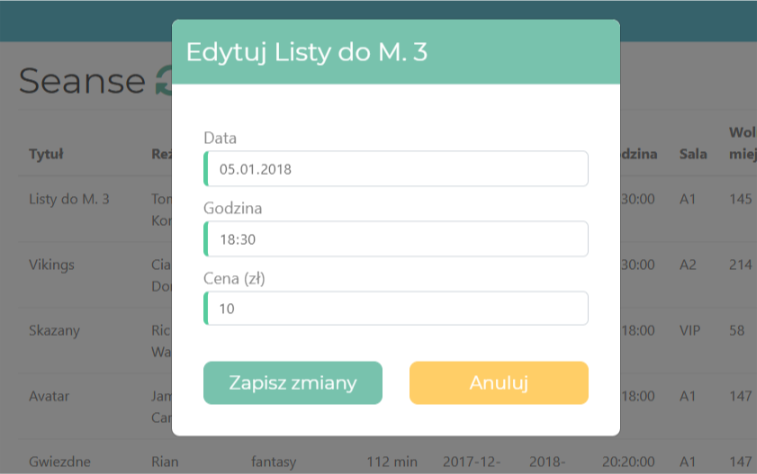
\includegraphics[width=1\linewidth]{rozdzial05/interfejs/edytujSeans.png}
	\caption{Edycja seansu}
	\label{fig:screen9}
\end{figure}

\begin{figure} [H]
	\centering
	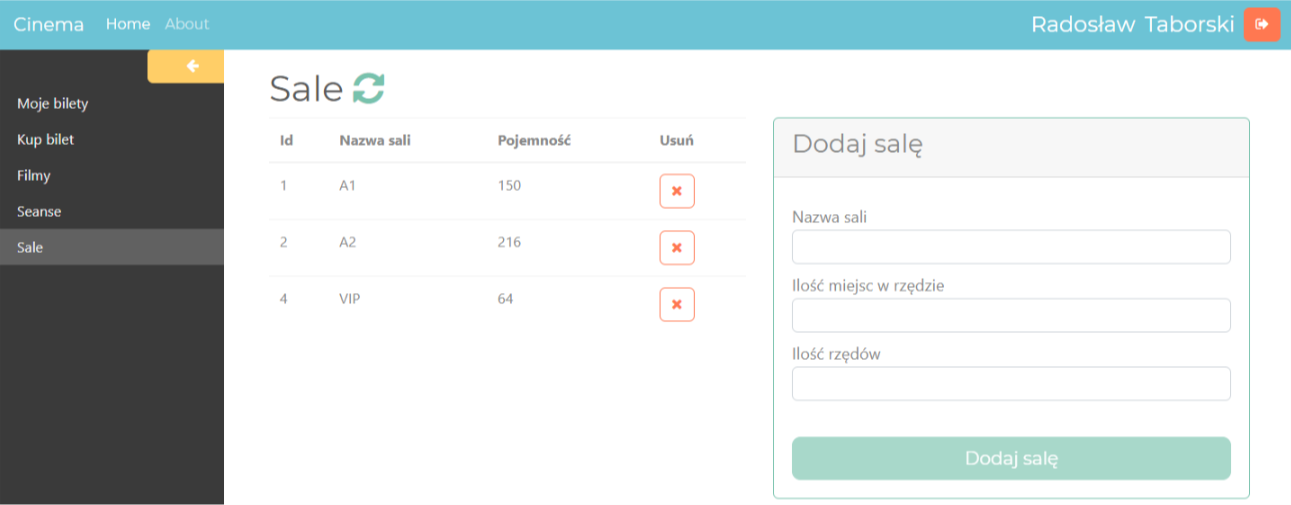
\includegraphics[width=1\linewidth]{rozdzial05/interfejs/sale.png}
	\caption{Widok sal dostępnych w kinie}
	\label{fig:screen10}
\end{figure}

Aplikacja również informuje o błędach z łącznością z serwerem (rysunek \ref{fig:alert2}) oraz o podaniu błędnego loginu lub hasła (rysunek \ref{fig:alert1})

\begin{figure} [H]
	\centering
	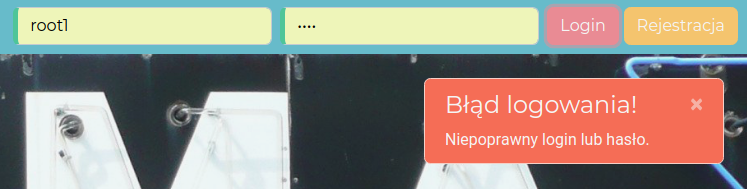
\includegraphics[width=1\linewidth]{rozdzial05/interfejs/alert1.png}
	\caption{Podanie błędnego loginu i hasła}
	\label{fig:alert1}
\end{figure}
		
\begin{figure} [H]
	\centering
	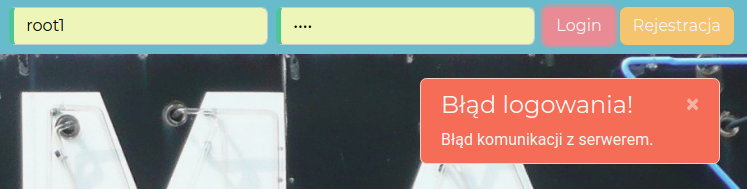
\includegraphics[width=1\linewidth]{rozdzial05/interfejs/alert2.png}
	\caption{Błąd komunikacji z serwerem}
	\label{fig:alert2}
\end{figure}

\section{Realizacja REST API}

REST (ang. Representational State Transfer) jest wzorcem narzucającym dobre praktyki tworzenia architektury aplikacji rozproszonych. RESTful Webservices (inaczej RESTful web API) jest usługą sieciową zaimplementowaną na bazie protokołu HTTP i głównych zasad wzorca REST. Ważnym założeniem REST jest istnienie zasobów (ang. resources) jako źródeł danych a także żądana akcja. API aplikacji zostało stworzone w postaci skryptu w PHP.

\begin{table}[H]
\centering

\label{restApi}
\begin{tabular}{|l|l|l|}
\hline
\textbf{zasób}                               & \textbf{metoda} & \textbf{zastosowanie}                \\ \hline
http://90.156.81.49:81/cinemaapi.php/filmy   & GET             & zostanie zwrócona lista filmów       \\ \hline
http://90.156.81.49:81/cinemaapi.php/filmy/1 & GET             & zostanie zwrócony film o id równym 1 \\ \hline
http://90.156.81.49:81/cinemaapi.php/film    & PUT             & dodanie nowego filmu                 \\ \hline
http://90.156.81.49:81/cinemaapi.php/film/1  & POST            & edycja filmu o id równym 1           \\ \hline
http://90.156.81.49:81/cinemaapi.php/film/1  & DELETE          & usunięcie filmu o id równym 1        \\ \hline
\end{tabular}
\caption{Przykładowe zastosowanie REST API}
\end{table}

Poniżej znajdują się fragmenty skryptu odpowiedzialnego za obsługę zapytań.

\lstinputlisting[captionpos=b,caption={Skrypt PHP API aplikacji},label={lst:api},basicstyle={\footnotesize\ttfamily}]{rozdzial05/cinemaApi.txt}

\lstinputlisting[captionpos=b,caption={Skrypt PHP obsługujący zapytania GET},label={lst:php},basicstyle={\footnotesize\ttfamily}]{rozdzial05/getApi.txt}